\documentclass[12pt]{article}
\usepackage[T1]{fontenc}
\usepackage[utf8]{inputenc}
\usepackage[margin=1in]{geometry}
\usepackage{times}
\usepackage{amsmath,amssymb}
\usepackage{graphicx}
\usepackage{booktabs}
\usepackage{natbib}
\usepackage[hidelinks]{hyperref}
\usepackage{caption}
\usepackage{microtype}
\usepackage{placeins}
\usepackage{float}
\bibliographystyle{apalike}
\newcommand{\GDPWeight}{94.2}
\newcommand{\BrazilWeight}{73.6}
\newcommand{\SingaporeWeight}{26.4}
\newcommand{\SCMPreRMSPE}{242}
\newcommand{\ASCMPreRMSPE}{238}
\newcommand{\PlaceboPre}{128}
\newcommand{\PlaceboPost}{605}
\newcommand{\SCMGapEnd}{26{,}541}
\newcommand{\ASCMGapEnd}{26{,}388}
\newcommand{\ObservedEnd}{1{,}781}
\newcommand{\SCMPathEnd}{28{,}322}
\newcommand{\ASCMPathEnd}{28{,}169}
\newcommand{\LOOMinGap}{16{,}860}
\newcommand{\LOOMaxGap}{26{,}541}
\newcommand{\ASCMNegativeMass}{1.37}
\newcommand{\SCMRatio}{2{,}412}
\newcommand{\ASCMRatio}{2{,}569}
\newcommand{\PlaceboHeldoutMean}{581}
\newcommand{\ASCMMinGapEnd}{28{,}562}
\newcommand{\ASCMMinPathEnd}{30{,}343}
\newcommand{\ASCMMinPreRMSPE}{190}
\newcommand{\PenaltyGapChange}{8.2}
\newcommand{\CVMinimumError}{96{,}433}
\newcommand{\CVOneSEError}{138{,}890}
\newcommand{\CVMinimumSE}{49{,}950}
\newcommand{\CVMinimumLambda}{4.25\times10^{5}}
\newcommand{\CVSelectedLambda}{6.74\times10^{8}}
\newcommand{\CVEligible}{21}
\newcommand{\MinimumNegativeMass}{28.19}
\newcommand{\SingaporeContribution}{17{,}055}
\newcommand{\SingaporeShare}{60.2}
\newcommand{\SingaporeGapEnd}{41{,}184}
\newcommand{\SpainGapEnd}{13{,}131}
\newcommand{\IndiaGapEnd}{10{,}134}
\newcommand{\SingaporePreRMSPE}{505}
\newcommand{\SingaporePostRMSPE}{14{,}329}
\newcommand{\NorthPostRMSPE}{11{,}881}
\newcommand{\SingaporeRatio}{805}


\begin{document}
\hypersetup{pageanchor=false}
\begin{titlepage}
\begin{center}
\vspace*{1.5cm}

{\Large\bfseries
One Peninsula, Two Destinies\\[0.4em]
A Synthetic Control Analysis of Korea's Economic Divergence\par
}

\vspace{1cm}

{\large
Kyungwook Back\textsuperscript{1,*}\quad
Sehun Bai\textsuperscript{1,*}\quad
Jungwoo Hong\textsuperscript{1,*}\par
}

\vspace{0.3cm}

{\small
\textsuperscript{1}Department of Statistics,
Korea University, Seoul, Korea\par
}

\vspace{1cm}
\textbf{Abstract}
\end{center}

\begingroup
\renewcommand{\thefootnote}{\fnsymbol{footnote}}
\footnotetext[1]{These authors contributed equally to this work.}
\endgroup
North and South Korea's economic divergence is often presented as evidence of the importance of institutions. We examine how its estimated magnitude depends on the historical comparison chosen for North Korea. Using reconstructed data, we fit standard and ridge-augmented synthetic controls and examine donor deletion and greater signed-weight extrapolation. Across the specifications examined, North Korea remains below its synthetic paths throughout the postwar period. The 2013 gaps range from approximately 17,000 to 29,000 international dollars per capita. Their size depends heavily on Singapore, whose high income contributes a large share of the synthetic northern outcome. The comparison yields a persistent negative gap, with the dollar estimate closely tied to the credibility of the donor countries used to construct it.

\vfill
\end{titlepage}
\setcounter{page}{1}
\hypersetup{pageanchor=true}

\section{Introduction}

\subsection{Institutions and the Korean comparison}
North and South Korea occupy a prominent place in arguments about the economic importance of institutions. Acemoglu, Johnson, and Robinson point to the two Koreas when contrasting central planning and collective ownership with private property and market exchange \citep[p.~1369]{acemoglu2001colonial}. The present difference in living standards gives that argument considerable force. A quantitative assessment still requires a view of how the northern economy might otherwise have developed.

The division occurred in a peninsula with regional differences in industrial structure, population, and economic activity. Liberation was followed by separate state formation, war, reconstruction, and different patterns of aid and trade. Those events shaped the institutions that emerged and the resources available to each economy. A comparison based only on the present North--South income gap absorbs this entire history. Reconstructing an alternative northern path requires closer attention to its starting position.

Our question is how far North Korea's observed GDP per capita departed from a path fitted to its pretreatment data. We build that path from other countries and examine how it changes under a different estimator and the removal of influential donors. This approach puts the choice of comparison economies and the quality of the historical fit at the center of the analysis.

\subsection{Policy motivation and previous work}
The economic consequences of division also matter for discussions of Korean unification. In the 2024 KINU Unification Survey, 52.9\% of respondents considered unification necessary \citep{kinu2024}. The economic questions surrounding integration are substantial. They concern the resources needed to raise northern living standards, the distribution of those costs, and the time over which gains might emerge.

Previous research has approached these questions with structural models. \citet{noland2000modeling} study Korean integration in a computable general equilibrium framework, examining trade, factor movements, and productivity changes. \citet{mckibbin2018modelling} use a dynamic model to compare reform, collapse, and crisis scenarios. Their construction of North Korea's input--output structure uses Vietnam's 2011 table as prior information. Such models make the integration process explicit, and their results depend on assumptions about migration, capital, productivity, and adjustment.

We examine a historical comparison that complements those prospective exercises. Synthetic control chooses a weighted combination of countries from the fit to pretreatment data. This replaces an individual comparison economy with an estimated donor mixture, while retaining choices about the donor set, predictors, and time window. The resulting gap describes an alternative historical trajectory under those choices. A forecast of future unification would additionally require a model of the integration process.

\subsection{Main findings}
Two results organize the paper. First, across every specification we examine, North Korea's observed GDP per capita stays below its synthetic path in all sixty postwar years, and the 2013 gap lies between roughly 17,000 and 29,000 international dollars per capita. Second, that range is wide for a reason that the diagnostics make visible. The synthetic unit matches North Korea on its colonial-era income level and on little else, and most of its 2013 value comes from Singapore. Shifting weight among the other donors barely moves the gap, while removing Singapore cuts it by more than a third. The sections that follow document both results. We argue that the first is well supported and that the second is the main limit on what the dollar figure means.

\section{Treatment and Estimation Design}

\subsection{Historical transition and observation periods}
The historical transition begins with liberation and division in 1945. North Korea subsequently nationalized much of production and adopted central planning. The comparison also incorporates war destruction, postwar reconstruction, aid, trade relationships, and later external shocks. The gap therefore concerns the historical path following division, with the contribution of each mechanism left unresolved.

The fitting period runs from 1911 to 1943, and the outcome comparison covers 1954 to 2013. We omit observations from 1944 through 1953. The software uses 1944 as the boundary immediately following the last fitting year. Excluding this interval avoids fitting to the years around liberation and war, while their lasting consequences remain in the later outcome series.

\subsection{Standard synthetic control}
Let $Y_{1t}$ denote North Korean GDP per capita and let $Y_{jt}$ denote donor outcomes for $j=2,\ldots,J+1$, with $J=9$. Standard synthetic control estimates donor weights by minimizing pretreatment predictor imbalance,
\begin{equation}
 \widehat w=\arg\min_{w\geq0,\;\boldsymbol{1}^{\mathsf T}w=1}
 (X_1-X_0w)^{\mathsf T}V(X_1-X_0w),
\end{equation}
where $X_1$ contains North Korean predictors and $X_0$ contains the corresponding donor predictors \citep{abadie2010synthetic}. The implementation scales predictor rows and selects the diagonal matrix $V$ using pretreatment GDP prediction error. We report $V$ alongside the balance table because it determines which mismatches receive most weight.

The fitted comparison is $\widehat Y_{1t}^{\mathrm{SCM}}=\sum_j\widehat w_jY_{jt}$. We define the annual gap as $G_t=Y_{1t}-\widehat Y_{1t}$. Negative values indicate GDP below the fitted comparison. Its interpretation depends on whether the donor relationship learned before division provides a useful approximation to the unobserved later path.

\subsection{Ridge augmentation}
We also estimate ridge-augmented synthetic control \citep{benmichael2021augmented}. It adjusts the initial weighted outcome for residual pretreatment imbalance using an outcome model,
\begin{equation}
 \widehat Y_{1t}^{\mathrm{ASCM}}
 =\sum_j\widehat w_jY_{jt}
 +\widehat m_t(X_1^{\mathrm{pre}})
 -\sum_j\widehat w_j\widehat m_t(X_j^{\mathrm{pre}}).
\end{equation}
Here $X_i^{\mathrm{pre}}$ denotes information from the fitting period, and $\widehat m_t$ predicts outcomes at time $t$. The ridge penalty regulates the adjustment. The initial SCM weights satisfy simplex constraints, and the final augmented representation can have signed donor weights.

We use the \texttt{Synth} and \texttt{augsynth} implementations. The standard model combines structural predictors with four averaged GDP blocks. The augmented model uses the same structural measures and the pretreatment GDP path. Its default penalty follows the package's one-standard-error rule, selecting the largest penalty with CV error within one SE of the minimum. We additionally fix the penalty at the CV minimum to examine sensitivity to greater extrapolation. The augmented fit has its own starting SCM weights, which differ from the standard estimator's weights because the inputs and weighting criterion differ.

\section{Data and Preprocessing}

\subsection{Historical series}
The working dataset combines GDP and population series with indicators from Clio Infra \citep{clioinfra2010} and the Maddison Project Database 2020 \citep{bolt2020maddison}. GDP levels are kept on the MPD 2020 scale of 2011 international dollars. Population is reported in thousands.

For the colonial period, the project assembled northern population values from peninsula and provincial records in the \textit{Statistical Yearbook of the Government-General of Korea} \citep{govgeneral1943}. The workbook also contains a reconstructed northern GDP series for 1911--1943. For the later period, growth estimates from \citet{chokim2020growth}, whose study covers 1956--1989, were linked to a Maddison benchmark. Per capita reconstruction additionally depends on population.

The workbook preserves the resulting early GDP values but does not retain all regional-allocation calculations or the complete 1954--1955 splice. These steps remain sources of measurement uncertainty. The analysis uses the archived values consistently across all estimators and donor checks.

\subsection{Donor countries and predictors}
The donor pool consists of Argentina, Brazil, Chile, Greece, India, Mexico, Portugal, Singapore, and Spain. South Korea is excluded because division and war directly shaped its path. Japan is excluded because Korean War procurement affected its economy. The remaining countries provide variation in income, agriculture, population, and institutions. Their subsequent histories also contain shocks, which motivates inspecting the fitted donor composition and deleting influential donors.

The structural predictors are population, cropland per capita, sulfur-dioxide emissions per capita, a livestock index, and adjusted education. For all ten countries, education years, cropland, sulfur-dioxide emissions, and each livestock count are recorded only in 1920, 1930, and 1940 within the main fitting period. Table~\ref{tab:availability} reports the nonmissing workbook entries for both fitting windows. Interpolation expands these sparse series to annual inputs without adding measurement dates.

\begin{table}[htbp]
\centering
\caption{Available workbook entries per country in the two fitting windows}
\label{tab:availability}
\small
\begin{tabular}{lrr}
\toprule
Workbook input & 1911--1943 & 1911--1934 \\
\midrule
Years of education & 3 & 2 \\
Cropland per capita & 3 & 2 \\
SO$_2$ emissions per capita & 3 & 2 \\
Each livestock count & 3 & 2 \\
Education Gini & 19--33 & 10--24 \\
Population & 29--33 & 22--24 \\
GDP per capita & 29--33 & 24 \\
\bottomrule
\end{tabular}

\caption*{\footnotesize Ranges describe differences across the ten countries. The first four rows use 1920, 1930, and 1940 for the main fit, and 1920 and 1930 for the 1935 placebo fit.}
\end{table}

We construct the livestock index as
\begin{equation}
 L_i=\frac{\mathrm{Cattle}_i+0.25\,\mathrm{Pigs}_i+0.10\,\mathrm{Goats}_i}
 {\mathrm{Population}_i},
\end{equation}
and adjusted education as
\begin{equation}
 H_i=\mathrm{Years\ of\ Education}_i
 \left(1-\frac{\mathrm{Education\ Gini}_i}{100}\right).
\end{equation}
The education Gini and population have more frequent entries, so the final education and livestock indices also vary through those inputs. Their sparse components remain based on the three benchmark dates. The standard fit also uses average GDP per capita in 1911--1920, 1921--1930, 1931--1940, and 1941--1943.

\subsection{Imputation within each fitting window}
We interpolate interior missing values linearly using calendar years and hold the nearest observed value constant at a segment's boundaries. Imputation is performed separately before and after the fitting cutoff. In the sparse benchmark series, the main fit copies the 1920 value to 1911--1919 and the 1940 value to 1941--1943. The 1935 placebo has only the 1920 and 1930 benchmarks, so 1931--1934 repeat the 1930 value. Each exercise starts again from the raw workbook. The structural averages in Table~\ref{tab:balance} are averages of these completed series.

This corrects the original workflow, which interpolated across the joined pre- and post-treatment periods after omitting 1944--1953. That workflow allowed later observations to enter some pretreatment covariates. All tables and figures below use the corrected preprocessing. Appendix~\ref{app:preprocessing} compares the two runs in the same software environment.

\section{Results}

\subsection{Donor weights and the pretreatment match}
The standard fit assigns \BrazilWeight\% of donor weight to Brazil and \SingaporeWeight\% to Singapore. The one-SE augmented fit retains those two as the largest contributors and gives a smaller positive weight to Portugal. Table~\ref{tab:weights} reports all final weights for these main fits. The ASCM negative weights have a combined absolute mass of \ASCMNegativeMass\%, so its final representation involves modest signed-weight extrapolation.

\begin{table}[htbp]
\centering
\caption{Estimated donor weights}
\label{tab:weights}
\small
\begin{tabular}{lrr}
\toprule
Country & SCM & ASCM (1-SE) \\
\midrule
Brazil & 0.73612 & 0.69664 \\
Singapore & 0.26388 & 0.25181 \\
Portugal & 0.00000 & 0.06104 \\
Mexico & 0.00000 & 0.00167 \\
Greece & 0.00000 & 0.00194 \\
Spain & 0.00000 & -0.00345 \\
Chile & 0.00000 & -0.00197 \\
India & 0.00000 & 0.00058 \\
Argentina & 0.00000 & -0.00826 \\
\bottomrule
\end{tabular}

\end{table}

Table~\ref{tab:balance} shows why the outcome fit and the structural match differ. The four GDP blocks receive \GDPWeight\% of the selected $V$ weight. As a result, the standard estimator gives substantially less penalty to mismatches in livestock, education, and population. Northern livestock is about 0.116 compared with 0.791 in the standard synthetic unit. The adjusted education values are about 0.018 and 0.393, while population is about 5.7 million and 23.8 million. Augmentation leaves appreciable differences in these predictors as well.

The $V$ weights are chosen to minimize pretreatment GDP prediction error. The resulting objective places much greater priority on GDP-block matching than on the structural predictors. Those predictors are sparsely measured, and the fit asks little of them. Figure~\ref{fig:prefit}(a) shows that the fitted GDP paths track the broad pretreatment rise, with discrepancies in individual years. Pretreatment RMSPE is \SCMPreRMSPE{} dollars for SCM and \ASCMPreRMSPE{} dollars for the default ASCM.

\begin{table}[htbp]
\centering
\caption{Pretreatment predictor balance and standard SCM predictor weights}
\label{tab:balance}
\footnotesize
\setlength{\tabcolsep}{3.5pt}
\begin{tabular}{lrrrrr}
\toprule
Predictor & Actual & SCM & ASCM & Donor mean & $V$ (\%) \\
\midrule
Livestock index & 0.1158 & 0.7909 & 0.7325 & 0.7000 & 0.9 \\
Adjusted education & 0.0178 & 0.3926 & 0.3918 & 1.2623 & 1.4 \\
Population (thousands) & 5,735 & 23,823 & 23,013 & 48,510 & 0.2 \\
SO$_2$ emissions per capita & 0.0016 & 0.0015 & 0.0014 & 0.0163 & 1.8 \\
Cropland per capita & 0.2489 & 0.3016 & 0.2933 & 0.6926 & 1.5 \\
GDP (1911--1920) & 1,261 & 1,352 & 1,348 & 2,604 & 33.0 \\
GDP (1921--1930) & 1,509 & 1,720 & 1,714 & 3,143 & 33.4 \\
GDP (1931--1940) & 2,162 & 1,969 & 1,975 & 3,195 & 16.3 \\
GDP (1941--1943) & 2,494 & 2,267 & 2,256 & 3,349 & 11.6 \\
\bottomrule
\end{tabular}

\caption*{\footnotesize GDP entries are block averages in 2011 international dollars. Structural entries average the completed 1911--1943 series. ASCM uses the final signed weights under the one-SE penalty.}
\end{table}

\FloatBarrier
\begin{figure}[H]
\centering
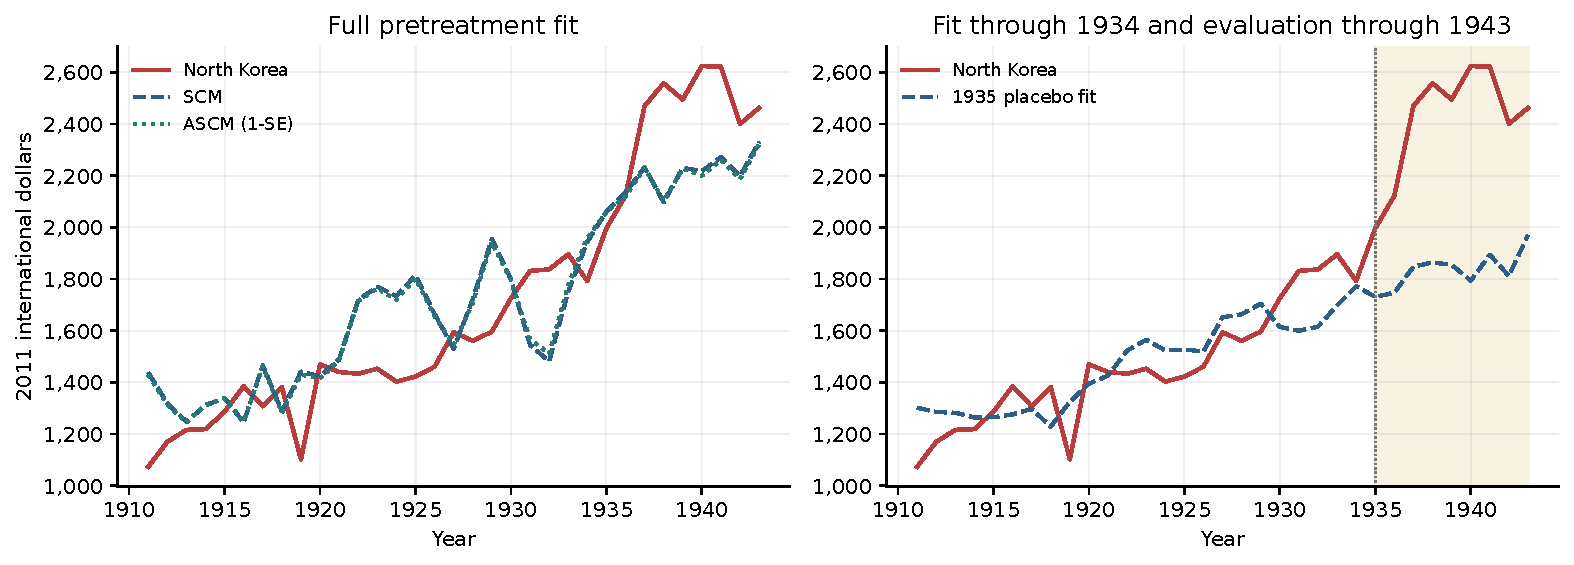
\includegraphics[width=\linewidth]{figures/pretreatment_and_1935.pdf}
\caption{Pretreatment fit and the 1935 placebo. Panel (a) uses the complete fitting period through 1943. Panel (b) fits through 1934 and evaluates the shaded years 1935--1943.}
\label{fig:prefit}
\end{figure}

\subsection{Long-run paths and annual differences}
Figure~\ref{fig:paths} compares the observed path with standard SCM and the one-SE augmented fit. North Korea's GDP remains below both synthetic paths in every observed year after 1953. The distance is relatively small during the early recovery years and widens from the 1970s onward. The observed series falls during the 1990s, while the donor-weighted paths continue to rise.

In 2013, observed GDP per capita is \ObservedEnd{} dollars. The standard comparison reaches \SCMPathEnd{} dollars and the augmented comparison \ASCMPathEnd{} dollars. The corresponding annual gaps are $-\SCMGapEnd$ and $-\ASCMGapEnd$ dollars. Table~\ref{tab:outcomes} reports selected years. These values describe the difference in income levels at each date.

\begin{figure}[H]
\centering
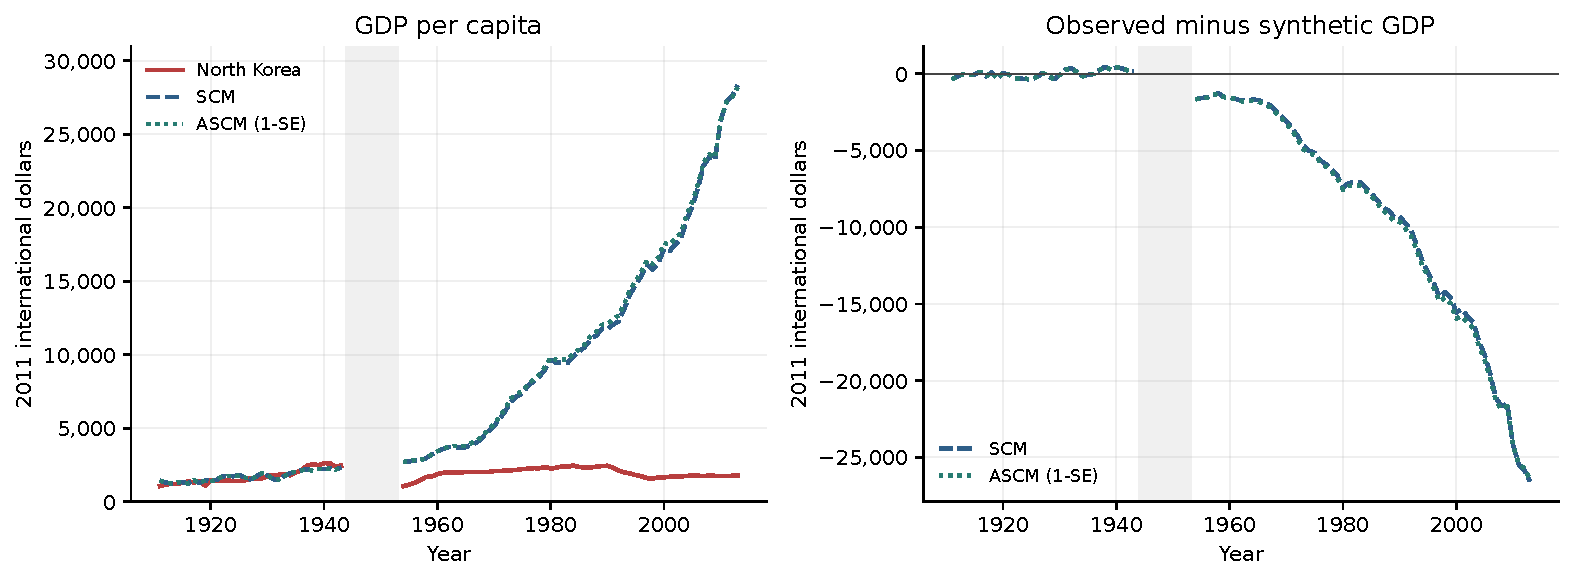
\includegraphics[width=\linewidth]{figures/paths_and_gaps.pdf}
\caption{Observed GDP per capita, standard SCM, and one-SE ASCM. The right panel shows the annual observed-minus-synthetic gaps. The shaded interval marks 1944--1953.}
\label{fig:paths}
\end{figure}

\begin{table}[H]
\centering
\caption{Observed GDP, standard SCM, and one-SE ASCM at selected dates}
\label{tab:outcomes}
\small
\setlength{\tabcolsep}{5pt}
\begin{tabular}{lrrrrr}
\toprule
Year & Actual & SCM path & ASCM path & SCM gap & ASCM gap \\
\midrule
1970 & 2,088 & 5,167 & 5,322 & -3,078 & -3,234 \\
1990 & 2,456 & 11,754 & 12,101 & -9,298 & -9,645 \\
2013 & 1,781 & 28,322 & 28,169 & -26,541 & -26,388 \\
\bottomrule
\end{tabular}

\caption*{\footnotesize All entries are in 2011 international dollars per capita.}
\end{table}

\subsection{The 1935 placebo and extrapolation}
We assign a placebo date in 1935 and refit the standard estimator using 1911--1934. The shortened fit uses three eight-year GDP blocks along with the five structural measures. Its evaluation period is 1935--1943, before the historical partition.

Figure~\ref{fig:prefit}(b) shows a clear positive gap in those nine evaluation years. RMSPE rises from \PlaceboPre{} dollars during fitting to \PlaceboPost{} dollars during evaluation, with an average held-out gap of \PlaceboHeldoutMean{} dollars. The fit ending in 1934 misses the northern acceleration in the late 1930s.

This result matters for the main comparison because its horizon extends for sixty years. Matching the full pretreatment period does not establish that the same relationship remains stable over that horizon. The placebo therefore shifts the interpretation toward the sign and broad scale of the later gap across the checked specifications. It gives little support for attaching precision to a particular long-run income level.



\subsection{Ridge penalty sensitivity}
The selected one-SE penalty is $\lambda=\CVSelectedLambda$, whereas the minimum CV error occurs at $\lambda=\CVMinimumLambda$. The estimated CV errors are \CVOneSEError{} and \CVMinimumError{}, respectively. The SE at the minimum is \CVMinimumSE{}, and all \CVEligible{} candidates in the search grid lie within one SE of that minimum. The curve therefore provides weak discrimination among penalties at the precision of this exercise. Appendix~\ref{app:placebo} displays the complete curve and its uncertainty.

The one-SE rule selects strong shrinkage within the uncertainty of the CV minimum. Here the resulting ridge correction changes the 2013 synthetic outcome by 148 dollars, about 0.6\% of its gap, and changes the post-period path by 58 dollars on average in absolute value. The final negative-weight mass is \ASCMNegativeMass\%. Table~\ref{tab:augmentation} separates standard SCM, ASCM's internal starting fit, and the two augmented fits.

\begin{table}[htbp]
\centering
\caption{ASCM starting fit and sensitivity to ridge penalty selection}
\label{tab:augmentation}
\small
\begin{tabular}{lrrr}
\toprule
Fit & Pre-RMSPE & 2013 synthetic & 2013 gap \\
\midrule
Standard SCM & 241.9 & 28,322 & -26,541 \\
ASCM initial & 243.5 & 28,021 & -26,240 \\
ASCM (1-SE) & 237.7 & 28,169 & -26,388 \\
ASCM (minimum CV) & 189.7 & 30,343 & -28,562 \\
\bottomrule
\end{tabular}

\caption*{\footnotesize All outcome entries are in 2011 international dollars per capita. Pretreatment RMSPE is an in-sample diagnostic.}
\end{table}

The minimum-CV fit allows substantially more outcome-model extrapolation. Its in-sample pretreatment RMSPE falls to \ASCMMinPreRMSPE{} dollars, accompanied by a larger negative-weight mass of \MinimumNegativeMass\%. The 2013 gap is $-\ASCMMinGapEnd$ dollars, \PenaltyGapChange\% larger in magnitude than the one-SE fit, and all sixty post-treatment gaps remain negative.

Table~\ref{tab:ridge_weights} shows how the additional flexibility changes the donor mixture. Portugal becomes the largest positive contributor and Brazil's weight is roughly halved. Spain and Argentina receive substantial negative weights, and Mexico also gains positive weight. The improved training fit thus comes with a markedly different signed-weight representation. We use this fit to examine sensitivity to greater extrapolation.

\begin{table}[htbp]
\centering
\caption{Final ASCM donor weights under the two penalty choices}
\label{tab:ridge_weights}
\small
\begin{tabular}{lrr}
\toprule
Country & ASCM (1-SE) & ASCM (minimum CV) \\
\midrule
Portugal & 0.0610 & 0.5832 \\
Brazil & 0.6966 & 0.3486 \\
Singapore & 0.2518 & 0.2468 \\
Spain & -0.0034 & -0.1380 \\
Mexico & 0.0017 & 0.1033 \\
Argentina & -0.0083 & -0.0643 \\
India & 0.0006 & -0.0344 \\
Chile & -0.0020 & -0.0277 \\
Greece & 0.0019 & -0.0176 \\
\bottomrule
\end{tabular}

\end{table}

The Brazil-led and Portugal-led fits yield 2013 gaps of approximately 26,000--29,000 dollars despite the redistribution of donor weights. Singapore's weight remains close to 0.25 under both penalties. Reshuffling the other donors moves the gap by a few thousand dollars, and Singapore's influence is untouched by this exercise.

\subsection{Placebos across countries}
We apply standard SCM and the one-SE ASCM to each donor. Figure~\ref{fig:placebo_gaps} displays all country-level gap paths. In 2013 the standard-SCM gaps are approximately $+\SingaporeGapEnd$ dollars for Singapore, $+\SpainGapEnd$ for Spain, $-\SCMGapEnd$ for North Korea, and $-\IndiaGapEnd$ for India. North Korea has the largest negative endpoint, while Singapore has the larger absolute endpoint. India also has negative gaps in all sixty post-1953 years under both estimators. Persistent negative gaps are therefore not unique to North Korea.

\begin{figure}[htbp]
\centering
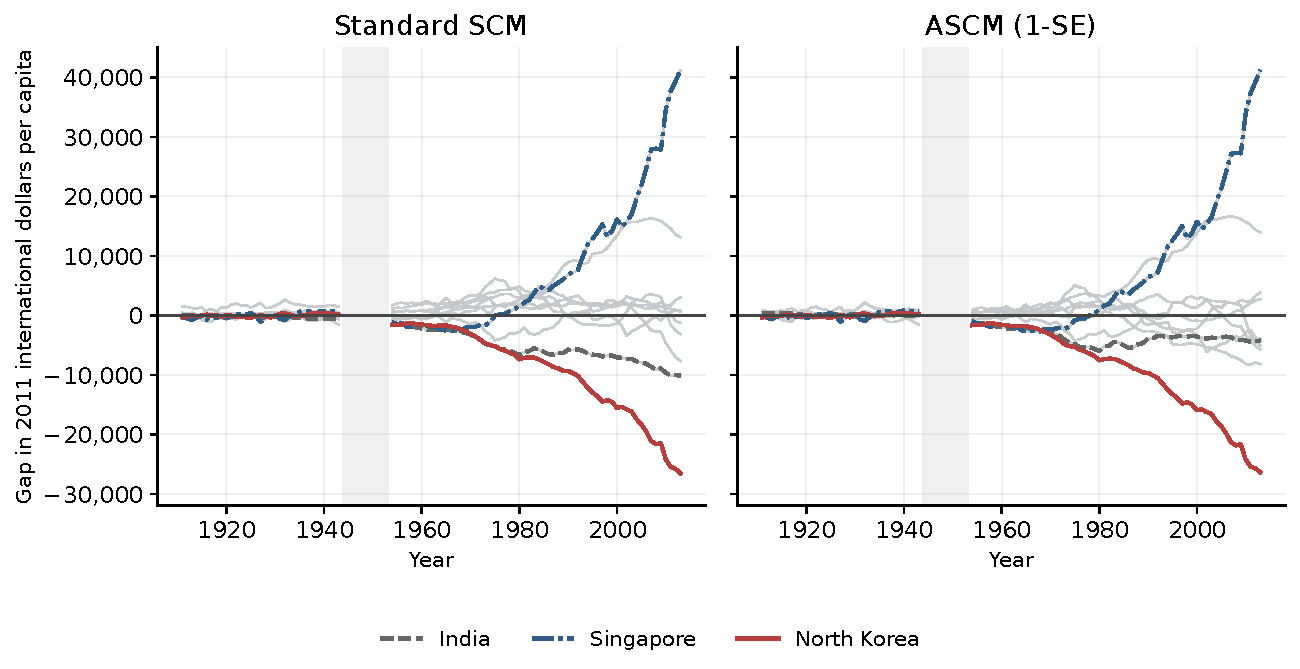
\includegraphics[width=\linewidth]{figures/placebo_gaps.pdf}
\caption{Complete country-level placebo gap paths. North Korea is red, Singapore is blue, India is dark grey, and the other seven donors are light grey. The ASCM panel uses the one-SE penalty. No donor is removed from either panel.}
\label{fig:placebo_gaps}
\end{figure}

The post/pre-MSPE ratios order these outcomes differently from their absolute errors. Under SCM, Singapore's post-period RMSPE is \SingaporePostRMSPE{} dollars, exceeding North Korea's \NorthPostRMSPE{} dollars. Its pretreatment RMSPE is also larger, at \SingaporePreRMSPE{} dollars compared with \SCMPreRMSPE{} dollars for North Korea. Normalization by pretreatment MSPE reverses their absolute-error ordering, giving ratios of \SingaporeRatio{} and \SCMRatio{}, respectively. North Korea's first rank reflects the increase relative to its small pretreatment error; Singapore's absolute deviation is the larger one. The corresponding ASCM ratio is \ASCMRatio{}, also the largest in its normalized comparison. The lower panels of Appendix Figure~\ref{fig:ratios} display both ratio distributions.

With nine donor placebos, its rank fraction is
\begin{equation}
 r=\frac{1+\sum_{j=2}^{10}\boldsymbol{1}\{R_j\geq R_1\}}{10}
 =0.10,
\end{equation}
where $R_i$ is the post/pre-MSPE ratio for unit $i$. This is the finest possible first rank in a ten-unit comparison. The main northern fit has nine controls, while each donor placebo uses the other eight donors and excludes North Korea. The rank is computed under that asymmetry.

Restricting placebos to pretreatment RMSPE at most five times the northern value removes Argentina from the SCM comparison. Its filtered rank fraction becomes $1/9\approx0.11$. The same rule retains all nine ASCM placebos, leaving its rank fraction at 0.10. We use the full donor set for the primary comparison.

\subsection{Deleting influential donors}
The corrected standard fit has two donors with weight above 0.001. We omit Brazil and Singapore in turn and refit both the donor and predictor weights. Figure~\ref{fig:loo} shows that the post-1953 synthetic path remains above the observed northern path in each case.

Singapore's role connects the placebo exercise to the main estimate. It has the largest post-period RMSPE in both placebo exercises, yet receives \SingaporeWeight\% of standard SCM donor weight. Its high 2013 income contributes \SingaporeContribution{} dollars, or \SingaporeShare\%, of synthetic North Korea's 2013 level. Thus a large component of the northern comparison comes from a country whose later path is poorly predicted by the remaining donors.

Removing Singapore and reoptimizing the weights reduces the 2013 gap from $-\LOOMaxGap$ to $-\LOOMinGap$ dollars. The negative direction survives, but the smaller endpoint shows how much the full estimate depends on Singapore's exceptional growth path within this donor pool. Because Singapore's weight rests on the GDP fit while its later path is the one the pool predicts worst, we read this Singapore-excluded figure as the more defensible anchor for the magnitude, and we return to that judgment in the conclusion. The two ridge penalties and the donor-deletion fits together produce 2013 gaps of roughly 17,000--29,000 dollars per capita.

\begin{figure}[htbp]
\centering
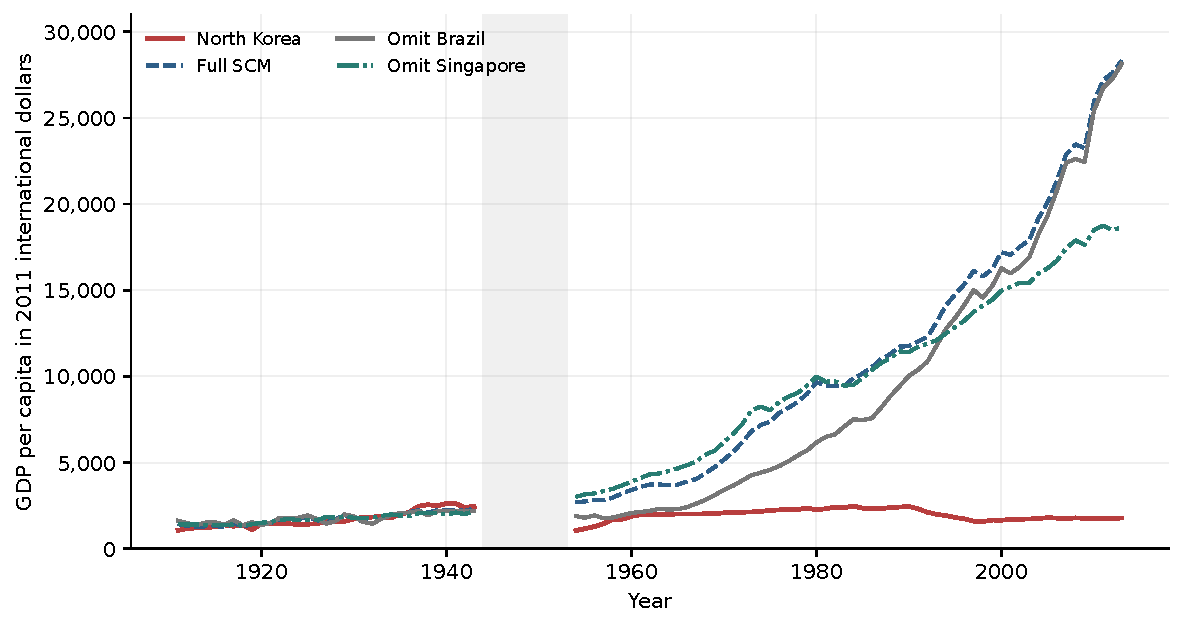
\includegraphics[width=.92\linewidth]{figures/donor_deletion.pdf}
\caption{Standard SCM after omitting each donor with baseline weight above 0.001. The full fit, both deletion fits, and observed North Korean GDP are shown.}
\label{fig:loo}
\end{figure}

\FloatBarrier
\section{Discussion and Conclusion}
The historical comparison gives a consistent answer about direction. Under standard SCM, both ridge-augmented fits, and both donor-deletion fits, North Korean GDP per capita lies below its synthetic path in every year from 1954 to 2013, and the distance widens from the 1970s onward. In 2013 the gap is between roughly 17,000 and 29,000 international dollars per capita, depending on the specification.

The diagnostics explain why we do not attach precision to any point in that range. The fit is driven almost entirely by colonial-era income levels. The GDP blocks carry \GDPWeight\% of the predictor weight, while education years, cropland, emissions, and the livestock counts are recorded at only three pretreatment dates, and the structural indicators built from them remain poorly balanced. A placebo cutoff in 1934 misses the late-1930s acceleration over a nine-year horizon, whereas the main comparison extends sixty years. The placebo exercise across donors gives North Korea the largest post/pre-MSPE ratio, but that rank reflects its small pretreatment error. In absolute terms Singapore deviates more, and India also shows sixty consecutive negative gaps. These checks support the sign and the broad scale of the divergence, and little beyond that.

What they leave open is the donor pool. Singapore receives about a quarter of the weight under every penalty choice and supplies about \SingaporeShare\% of synthetic North Korea's 2013 income. It earns that weight through the pretreatment GDP fit that dominates the weight selection. The synthetic unit assembled around it still carries several times North Korea's livestock, education, and population levels. Colonial North Korea was an agrarian territory with Japanese-built heavy industry and hydroelectric capacity. Singapore was an entrep\^ot city-state without a hinterland, and its growth after 1965 is the path that our own placebo exercise predicts worst from the remaining donors. We do not find that path a credible description of what a market-oriented North Korea would have done, and we read the Singapore-excluded figure of about 17,000 dollars as the more defensible anchor for the magnitude. The larger figures show what the method produces when the GDP fit alone decides which donors enter. The divergence is large under any of these readings. Putting a number on it turns out to depend on which histories North Korea could plausibly have shared, and that is a question about history as much as about estimation.

\section*{Statement of AI Usage}
AI tools assisted with translation of Korean-language sources, bibliographic searches, reference summaries, conceptual discussions, code debugging, and language editing. The authors are responsible for the data, calculations, citations, and conclusions.

\appendix
\section{Effect of the Preprocessing Correction}
\label{app:preprocessing}
We replayed the original joined-period imputation and the corrected cutoff-specific imputation in the same R environment. The replay reproduces the originally reported SCM and ASCM donor weights at their displayed precision. The corrected standard fit shifts weight from Portugal toward Brazil and Singapore. The augmented fit changes less. Table~\ref{tab:processing} compares pretreatment RMSPE and the final annual gap.

\begin{table}[htbp]
\centering
\caption{Original and corrected imputation in the same software environment}
\label{tab:processing}
\small
\begin{tabular}{lrrr}
\toprule
Model & Imputation & Pre-RMSPE & 2013 gap \\
\midrule
SCM & Original & 252.8 & -24,741 \\
SCM & Corrected & 241.9 & -26,541 \\
ASCM & Original & 249.5 & -25,803 \\
ASCM & Corrected & 237.7 & -26,388 \\
\bottomrule
\end{tabular}

\caption*{\footnotesize Gaps and RMSPE are in 2011 international dollars per capita. The main text uses the corrected runs.}
\end{table}

As a direct check on the correction, we multiplied observations after each cutoff by ten and repeated preprocessing. Pretreatment inputs remained unchanged for the 1944 main cutoff and the 1935 placebo cutoff. All nine donor placebos for each estimator and both donor-deletion fits completed successfully. The code bundle records the input fingerprint, configuration, complete result tables, and software versions.

\FloatBarrier
\clearpage
\section{Penalty Selection and Placebo Ratios}
\label{app:placebo}
Figure~\ref{fig:cv} shows the default ASCM cross-validation curve. The minimum estimated error is \CVMinimumError{}, with a fold-based SE of \CVMinimumSE{}. The one-SE rule chooses the strongest penalty in the grid because its error of \CVOneSEError{} is still below the eligibility threshold. Every candidate falls within this threshold. The estimated losses vary across the grid, while their uncertainty leaves the tuning exercise weakly discriminating among penalties.

\begin{figure}[htbp]
\centering
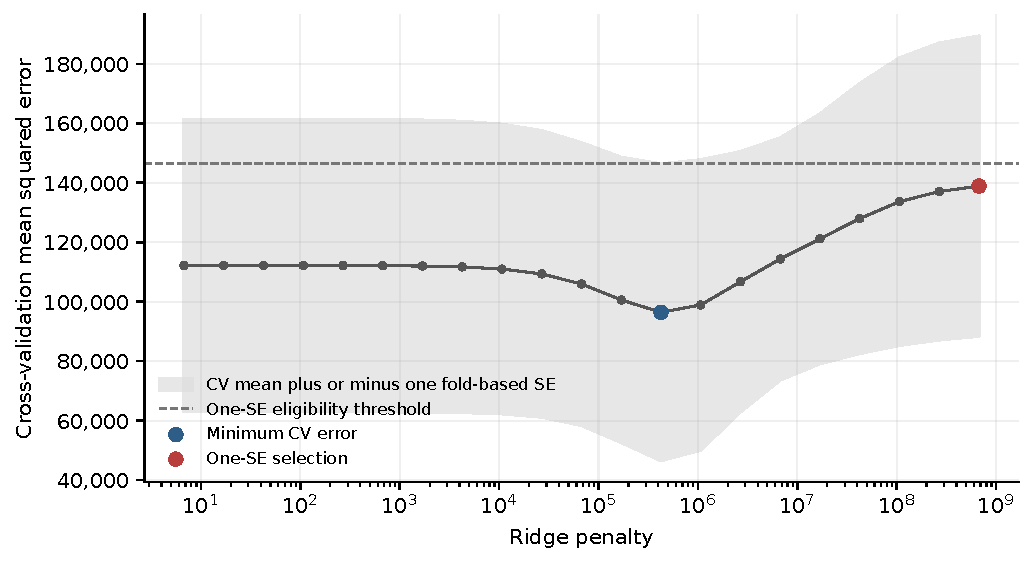
\includegraphics[width=.80\linewidth]{figures/ridge_cv.pdf}\\[0.8em]
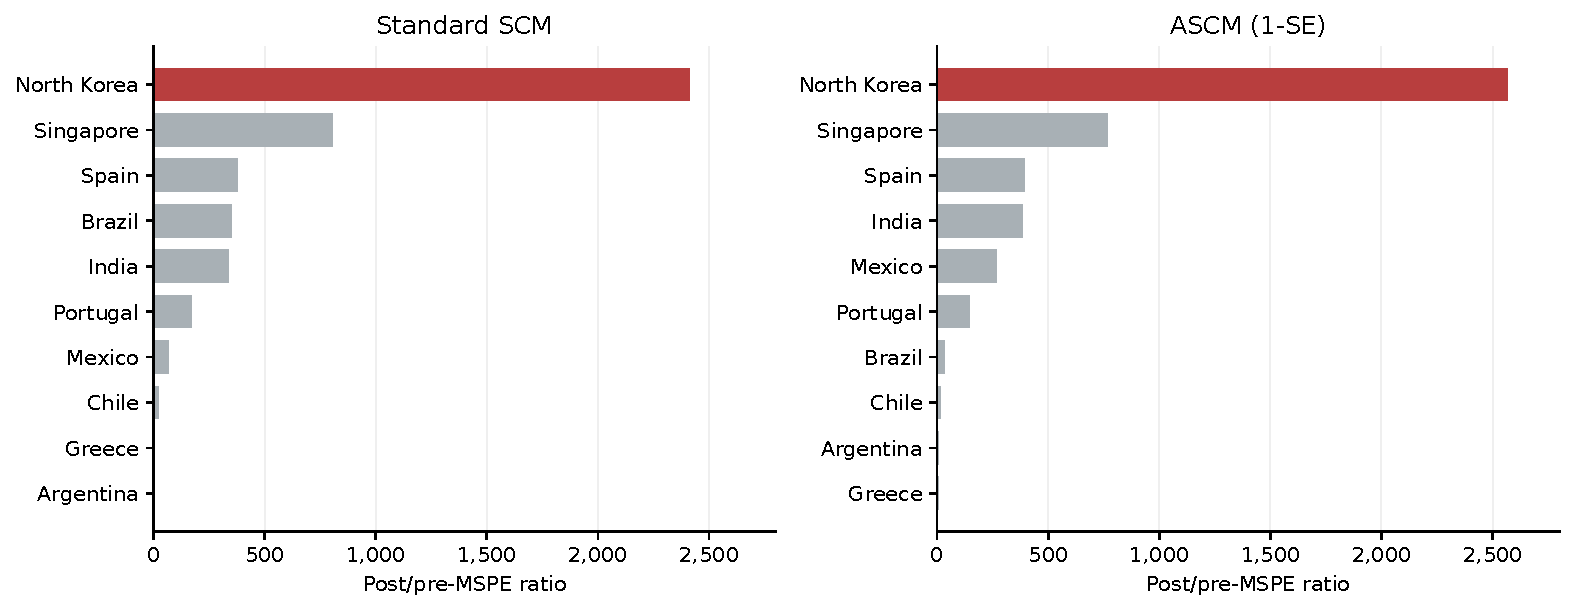
\includegraphics[width=.92\linewidth]{figures/placebo_ratios.pdf}
\caption{Penalty selection and normalized placebo errors. The upper panel shows the CV mean with one fold-based SE and the one-SE eligibility threshold. Markers identify the minimum-error and one-SE choices. The lower panels show post/pre-MSPE ratios for all ten units. ASCM uses the one-SE penalty, and North Korea's rank fraction is 0.10 in each comparison.}
\label{fig:cv}
\label{fig:ratios}
\end{figure}

\FloatBarrier
\clearpage
\bibliography{scm_references}
\end{document}
